
\chapter{Fruitful Subroutines}
\label{fruitchap}

Most of the Perl functions we have used, such as the math
functions, produce return values.  But most of the subroutines 
we've written so far are void: they have an effect, like 
printing a value, but they don't have a return value.  In
this chapter you will learn to write fruitful functions.


\section{Return Values}
\index{return!value}

Calling a fruitful function generates a return value, 
which we usually assign to a variable or use as part 
of an expression:

\begin{verbatim}
my $pi = 4 * atan 1;
my $height = $radius * sin $radians;
\end{verbatim}
%
Many of the subroutines we have written so far are void.  
Speaking casually, they have no usable return value; more 
precisely, their return value may be {\tt Any}, {\tt Nil}, 
{\tt ()}, or {\tt True}.

In this chapter, we are (finally) going to write fruitful subroutines.
The first example is {\tt area}, which returns the area of a circle
with the given radius:

\begin{verbatim}
sub area($radius) {
    my $circular_area = pi * $radius**2;
    return $circular_area;
}
\end{verbatim}
%
We have seen the {\tt return} statement before, but in a fruitful
function the {\tt return} statement includes
an expression.  This statement means: ``Return immediately from
this function and use the following expression as a return value.''
The expression can be arbitrarily complicated, so we could
have written this function more concisely:
\index{return!statement}
\index{statement!return}

\begin{verbatim}
sub area($radius) {
    return pi * $radius**2;
}
\end{verbatim}
%
On the other hand, {\bf temporary variables} like 
\verb'$circular_area' can make debugging easier. They 
may also help document what is going on.
\index{temporary variable}
\index{variable!temporary}

Sometimes it is useful to have multiple return statements, for 
example one in each branch of a conditional:

\begin{verbatim}
sub absolute_value($num){
    if $num < 0 {
        return -$num;
    } else {
        return $num;
    }
}
\end{verbatim}
%
Since these {\tt return} statements are in an alternative 
conditional, only one runs.

This could also be written more concisely using the statement 
modifier syntax:

\begin{verbatim}
sub absolute_value($num){
    return -$num if $num < 0;
    return $num;
}
\end{verbatim}
%
Here again, only one of the return statements runs: if the 
number is negative, the first return statement is executed and 
the subroutine execution stops there; if the number is 
positive or zero, then only the second return statement is 
executed. 

As soon as a return statement runs, the function
terminates without executing any subsequent statements.
Code that appears after an unconditional {\tt return} statement, 
or any other place the flow of execution can never reach, 
is called {\bf dead code}.
\index{dead code}

In a fruitful function, it is a good idea to ensure
that every possible path through the program hits a
{\tt return} statement.  For example:

\begin{verbatim}
# WARNING: faulty code
sub absolute_value($num){
    if $num < 0 {
        return -$num;
    } 
    if $num > 0 {
        return $num;
    }
}
\end{verbatim}
%


This subroutine is incorrect because if {\tt \$num} happens to be 0,
neither condition is true, and the subroutine ends without hitting a
{\tt return} statement.  If the flow of execution gets to the end
of a function, the return value is {\tt ()}, which basically 
means ``not defined'' and is clearly not the absolute value of 0:
\index{undefined value}

\begin{verbatim}
> absolute_value(0)
()
\end{verbatim}
%
By the way, Perl provides a built-in function called 
{\tt abs} that computes absolute values.
\index{abs function or method}
\index{function!abs}

\label{compare}
As an exercise, write a {\tt compare} subroutine that 
takes two numbers, {\tt \$x} and {\tt \$y}, and returns {\tt 1} 
if {\tt \$x > \$y}, {\tt 0} if {\tt \$x == \$y}, and 
{\tt -1} if {\tt \$x < \$y}.

Solution: \ref{sol_compare}
\index{compare function}
\index{function!compare}


\section{Incremental Development}
\label{incremental.development}
\index{development plan!incremental}
\index{incremental development}

As you write larger functions, you might find yourself
spending more time debugging.

To deal with increasingly complex programs,
you might want to try a process called
{\bf incremental development}.  The goal of incremental development
is to avoid long debugging sessions by adding and testing only
a small amount of code at a time.
\index{testing!incremental development}
\index{Pythagorean theorem}

As an example, suppose you want to find the distance between 
two points, given by the Cartesian or rectangular coordinates 
$(x_1, y_1)$ and $(x_2, y_2)$. By the Pythagorean theorem, 
the distance is:
\index{Pythagorean theorem}
\index{Cartesian coordinates}
\index{coordinates!Cartesian}
\index{rectangular!coordinates}
\index{coordinates!rectangular}


\begin{displaymath}
\mathrm{distance} = \sqrt{(x_2 - x_1)^2 + (y_2 - y_1)^2}
\end{displaymath}
%
The first step is to consider what a {\tt distance} function should
look like in Perl.  In other words, what are the inputs (parameters)
and what is the output (return value)?

In this case, the inputs are two points, which you can represent
using four numbers.  The return value is the distance represented by
a numeric value.

Immediately you can write an outline of the function:

\begin{verbatim}
sub distance($x1, $y1, $x2, $y2) {
    return 0.0;
}
\end{verbatim}
%
Obviously, this version doesn't compute distances; it always returns
zero.  But it is syntactically correct, and it runs, which means that
you can test it before you make it more complicated.

To test the new function, call it with sample arguments:

\begin{verbatim}
> distance(1, 2, 4, 6);
0.0
\end{verbatim}
%
I chose these values so that the horizontal distance is 3 and the
vertical distance is 4; that way, the result is 5, the hypotenuse 
of a 3-4-5 triangle. When testing a function, it is
useful to know the right answer.
\index{testing!knowing the answer}

At this point we have confirmed that the function is syntactically
correct, and we can start adding code to the body.
A reasonable next step is to find the differences
$x_2 - x_1$ and $y_2 - y_1$.  The next version stores those values in
temporary variables and prints them:

\begin{verbatim}
sub distance($x1, $y1, $x2, $y2) {
    my $dx = $x2 - $x1;
    my $dy = $y2 - $y1;
    say '$dx is', $dx;
    say '$dy is', $dy;
    return 0.0;
}
\end{verbatim}
%
If the function is working, it should display \verb"$dx is 3" and 
\verb"$dy is 4" (and still return 0.0).  If so, we know that the 
function is getting the right arguments and performing the 
first computation correctly.  If not, there are only a few lines 
to check.

Next we compute the sum of squares of {\tt \$dx} and {\tt \$dy}:

\begin{verbatim}
sub distance($x1, $y1, $x2, $y2) {
    my $dx = $x2 - $x1;
    my $dy = $y2 - $y1;
    my $dsquared = $dx**2 + $dy**2;
    say '$dsquared is: ', $dsquared;
    return 0.0;
}
\end{verbatim}
%
Again, you would run the program at this stage and check the output
(which should be 25).
Finally, you can use the {\tt sqrt} built-in function to compute 
and return the result:
\index{sqrt function}
\index{function!sqrt}

\begin{verbatim}
sub distance($x1, $y1, $x2, $y2) {
    my $dx = $x2 - $x1;
    my $dy = $y2 - $y1;
    my $dsquared = $dx**2 + $dy**2;
    my $result = sqrt $dsquared;
    return $result;
}
\end{verbatim}
%
If that works correctly, you are done.  Otherwise, you might
want to print the value of {\tt \$result} before the return
statement.

The final version of the subroutine doesn't display anything when it
runs; it only returns a value.  The {\tt print} statements we wrote
are useful for debugging, but once you get the function working, you
should remove them.  Code like that is sometimes called 
{\bf scaffolding} because it is helpful for building the program 
but is not part of the final product.
\index{scaffolding}

When you start programming, you should add only a line or two of code at a
time.  As you gain more experience, you might find yourself writing
and debugging bigger chunks.  Either way, incremental development
can save you a lot of debugging time.

The key aspects of the process are:

\begin{enumerate}

\item Start with a working program and make small incremental changes. 
At any point, if there is an error, you should have a good idea
where it is.

\item Use variables to hold intermediate values so you can
display and check them.

\item Once the program is working, you might want to remove some of
the scaffolding or consolidate multiple statements into compound
expressions, but only if doing so does not make the program 
difficult to read.

\end{enumerate}

Note that, at least for relatively simple cases, you can also 
use the REPL to test expressions and even multiline statements 
or subroutines in interactive mode before you commit them to your 
program code. This is usually fast and can save you some time.
\index{REPL}
\index{interactive mode}

\label{hypotenuse}
As an exercise, use incremental development to write a function
called {\tt hypotenuse} that returns the length of the hypotenuse of a
right triangle given the lengths of the other two legs as arguments.
Record each stage of the development process as you go.

Solution: \ref{sol_hypotenuse}.
\index{hypotenuse}



\section{Composition}
\index{composition}
\index{function composition}

As you should expect by now, you can call one function from within
another.  As an example, we'll write a function that takes two points,
the center of the circle and a point on the perimeter, and computes
the area of the circle.

Assume that the center point is stored in the variables {\tt \$x-c} and
{\tt \$y-c}, and the perimeter point is in {\tt \$x-p} and {\tt \$y-p}. The
first step is to find the radius of the circle, which is the distance
between the two points.  We just wrote a function, {\tt
distance}, that does that:

\begin{verbatim}
my $radius = distance($x-c, $y-c, $x-p, $y-p);
\end{verbatim}
%
The next step is to find the area of a circle with that radius;
we just wrote that, too:

\begin{verbatim}
my $result = area($radius);
\end{verbatim}
%
Encapsulating these steps in a function, we get:
\index{encapsulation}

\begin{verbatim}
sub circle-area($x-c, $y-c, $x-p, $y-p) {
    my $radius = distance($x-c, $y-c, $x-p, $y-p);
    my $result = area($radius)
    return $result;
}
\end{verbatim}
%
The temporary variables {\tt \$radius} and {\tt \$result} are useful for
development and debugging, but once the program is working, we can
make it more concise by composing the function calls:

\begin{verbatim}
sub circle-area($x-c, $y-c, $x-p, $y-p) {
    return area distance($x-c, $y-c, $x-p, $y-p);
}
\end{verbatim}
%

The last line of the previous example now works like a data 
pipeline from right to left: the \verb'distance' function 
takes the four arguments and returns a distance (the radius) 
which is fed as an argument to the \verb'area'; with this 
argument, \verb'area' is now able to return the area, which 
is then returned by \verb'circle-area' to the caller code. 
We'll come back later to this very expressive data pipeline 
model.
\index{pipe-line programming}

\section{Boolean Functions}
\label{boolean}

Functions can return Boolean values, which is often convenient for hiding
complicated tests inside functions. For example:
\index{Boolean function} 

\begin{verbatim}
sub is-divisible(Int $x, Int $y) {
    if $x % $y == 0 {
        return True;
    } else {
        return False;
    }
}
\end{verbatim}
%
It is common to give Boolean functions names that sound like yes/no
questions; \verb"is-divisible", for instance, returns either 
{\tt True} or {\tt False} to indicate whether {\tt x} is 
divisible by {\tt y}.

Here is an example:

\begin{verbatim}
> is-divisible(6, 4);
False
> is-divisible(6, 3);
True
\end{verbatim}
%
The result of the {\tt ==} operator is a Boolean value, so we 
can write the subroutine more concisely by returning it directly:

\begin{verbatim}
sub is-divisible(Int $x, Int $y) {
    return $x % $y == 0
}
\end{verbatim}
%
If there is no return statement, a Perl subroutine returns the 
value of expression on the last code line of the subroutine 
(provided the last code line is an expression that gets evaluated), so that the 
{\tt return} statement is not required here. In addition, 
since 0 is a false value and any other integer a true value, 
this could be further rewritten as follows:
\begin{verbatim}
sub is-divisible(Int $x, Int $y) { 
    not $x % $y 
}
\end{verbatim}

The {\tt Int} type declarations in the subroutine signatures above 
are not necessary. The subroutine would work without them, but 
they can provide some form of protection against using this 
subroutine with faulty arguments.

Boolean functions are often used in statement modifiers:
\index{statement modifier}
\index{modifier!statement}

\begin{verbatim}
say "$x is divisible by $y" if is-divisible($x, $y);
\end{verbatim}
%
It might be tempting to write something like:

\begin{verbatim}
say "$x is divisible by $y" if is-divisible($x, $y) == True;
\end{verbatim}
%
But the extra comparison is unnecessary: {\tt is-divisible} 
returns a Boolean value that can be interpreted directly by
the {\tt if} conditional.

\label{isbetween}
As an exercise, write a function \verb"is-between(x, y, z)" that
returns {\tt True} if $x \le y \le z$ or {\tt False} otherwise.

Solution: \ref{sol_isbetween}.

\section{A Complete Programming Language}

We've seen in the section above several ways of writing a 
subroutine to check the divisibility of two integers.
\index{divisibility}

In fact, as briefly mentioned earlier, Perl~6 has a 
``is divisible'' operator, \verb'%%', which returns 
{\tt True} if the number on the left is divisible by 
the one on the right:
%\index{%%!is divisible operator}
\index{is divisible operator}

\begin{verbatim}
> 9 %% 3
True
> 9 %% 4
False
\end{verbatim}

So there was no need to write the {\tt is-divisible} subroutine. 
But don't worry, that's all right if you did not remember that. 
Speakers of natural languages are allowed to have different 
skill levels, to learn as they go and to put the language 
to good use before they know the whole language. The same 
is true with Perl. You (and I) don't know all about Perl~6 
yet, just as we don't know all of English. But it is in fact 
``Officially Okay in Perl Culture'' to use the subset of 
the language that you know. You are in fact 
encouraged to use what is sometimes called ``baby Perl'' 
to write programs, even if they are somewhat clumsy at the 
beginning. That's the best way of learning Perl, just as using 
``baby talk'' is the right way for a child to learn English.
\index{baby Perl}
\index{Perl culture}

The number of different ways of accomplishing a given task, 
such as checking whether one number is divisible 
by another, is an example of one of Perl's mottos: 
\emph{there is more than 
one way to do it}, oft abbreviated TIMTOWTDI. Some ways may be 
more concise or more efficient than others, but, in the Perl 
philosophy, you are perfectly entitled to do it your way, 
especially if you're a beginner, provided you find the correct 
result.
\index{there is more than one way to do it}
\index{TIMTOWTDI}
\index{Turing!complete language}
\index{language!Turing complete}
\index{Turing, Alan}
\index{Turing!thesis}

We have only covered a small subset of Perl~6 so far, but you 
might be interested to know that this subset is a {\em complete}
programming language, which means that essentially anything 
that can be computed can be expressed in this language.  
Any program ever written could be rewritten using only the 
language features you have learned so far (actually, you 
would need a few commands to control devices like the mouse, 
disks, networks, etc., but that's all).

Proving that claim is a nontrivial exercise first accomplished by Alan
Turing, one of the first computer scientists (some would argue that he
was a mathematician, but a lot of early computer scientists started as
mathematicians).  Accordingly, it is known as the Turing Thesis.
For a more complete (and accurate) discussion of the Turing Thesis,
I recommend Michael Sipser's book {\em Introduction to the
Theory of Computation}.

\section{More Recursion}
\label{more.recursion}
\index{recursion}


To give you an idea of what you can do with the tools you have learned
so far, we'll evaluate a few recursively defined mathematical
functions.  A recursive definition is similar to a circular
definition, in the sense that the definition contains a reference to
the thing being defined.  A truly circular definition is not very
useful:

\begin{description}

\item[Vorpal] An adjective used to describe something that is vorpal.
\index{vorpal}
\index{circular definition}
\index{definition!circular}

\end{description}

If you saw that definition in the dictionary, you might be annoyed. On
the other hand, if you looked up the definition of the factorial
function, denoted with the symbol $!$, you might get something like
this:
%
\begin{eqnarray*}
&&  0! = 1 \\
&&  n! = n (n-1)!
\end{eqnarray*}
%
This definition says that the factorial of 0 is 1, and the 
factorial of any other (positive integer) value, $n$, is 
$n$ multiplied by the factorial of $n-1$.

So $3!$ is 3 times $2!$, which is 2 times $1!$, which is 1 times
$0!$. Putting it all together, $3!$ equals 3 times 2 times 1 times 1,
which is 6.
\index{factorial!function}
\index{function!factorial}
\index{recursive definition}

If you can write a recursive definition of something, you can
write a Perl program to evaluate it. The first step is to decide
what the parameters should be.  In this case it should be clear
that {\tt factorial} takes a number\footnote{It should really be an 
integer, but we'll get back to that later in this chapter.}:

\begin{verbatim}
sub factorial($n){
}
\end{verbatim}
%
If the argument happens to be 0, all we have to do is return 1:

\begin{verbatim}
sub factorial($n){
    if $n == 0 {
        return 1;
    }
}   
\end{verbatim}
%
Otherwise, and this is the interesting part, we have to make a
recursive call to find the factorial of $n-1$ and then 
multiply it by $n$:
\index{factorial!using recursion}

\begin{verbatim}
sub factorial($n){
    if $n == 0 {
        return 1;
    } else {
        my $recurse = factorial($n-1);
        my $result = $n * $recurse;
        return $result;
    }
}
\end{verbatim}
%
The flow of execution for this program is similar to the flow of {\tt
countdown} in Section~\ref{recursion}.  If we call {\tt factorial}
with the value 3:

Since 3 is not 0, we take the second branch and calculate the factorial
of {\tt \$n-1}...

\begin{quote}
Since 2 is not 0, we take the second branch and calculate the factorial of
{\tt \$n-1}...


  \begin{quote}
  Since 1 is not 0, we take the second branch and calculate the factorial
  of {\tt \$n-1}...


    \begin{quote}
    Since 0 equals 0, we take the first branch and return 1
    without making any more recursive calls.
    \end{quote}


  The return value, 1, is multiplied by \verb'$n', which is 1, and the
  result is returned.
  \end{quote}


The return value, 1, is multiplied by \verb'$n', which is 2, and the
result is returned.
\end{quote}


The return value, 2, is multiplied by \verb'$n', which is 3, and 
the result, 6, becomes the return value of the subroutine call 
that started the whole process.
\index{stack diagram}

Figure~\ref{fig.stack3} shows what the stack diagram looks like for
this sequence of function calls.

\begin{figure}
\centerline
{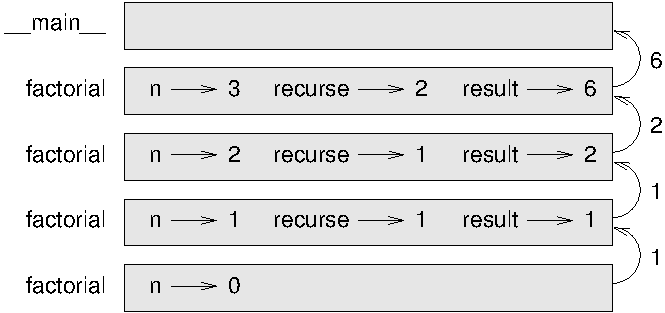
\includegraphics[scale=0.8]{figs/stack3.pdf}}
\caption{Stack diagram.}
\label{fig.stack3}
\end{figure}

The return values are shown being passed back up the stack.  In each
frame, the return value is the value of {\tt result}, which is the
product of {\tt n} and {\tt recurse}.
\index{function!frame}
\index{frame}

In the last frame, the local
variables {\tt recurse} and {\tt result} do not exist, because
the branch that creates them does not run.

A seasoned Perl programmer might write a more concise or
more idiomatic subroutine\footnote{We will see later even 
more idiomatic ways of computing the factorial of a number.}:
\index{idiomatic}

\begin{verbatim}
sub factorial($n){
    return 1 if $n == 0;
    return $n * factorial $n-1;
}
\end{verbatim}
%
This is not better than our initial version, and will probably 
not run significantly faster, but this is arguably clearer, 
at least once you get used to this type of syntax.

\section{Leap of Faith}
\index{recursion}
\index{leap of faith}

Following the flow of execution is one way to read programs, but
it can quickly become overwhelming.  An alternative is what may 
be called the ``leap of faith.''  When you come to a
subroutine call, instead of following the flow of execution, you {\em
assume} that the subroutine works correctly and returns the right
result.

In fact, you are already practicing this leap of faith when you use
built-in functions.  When you call math functions such as {\tt cos} or {\tt sqrt},
you don't examine the bodies of those functions.  You just
assume that they work because the people who wrote the built-in
functions were likely to be good programmers (and because you 
can safely assume that they have been thoroughly tested).

The same is true when you call one of your own subroutines.  For
example, in Section~\ref{boolean}, we wrote a subroutine called 
\verb"is-divisible" that determines whether one number is divisible by
another.  Once we have convinced ourselves that this subroutine is
correct---by examining the code and testing---we can use the subroutine without looking at the body again.
\index{testing!leap of faith}

The same is true of recursive programs.  When you get to the recursive
call, instead of following the flow of execution, you should assume
that the recursive call works (returns the correct result) and then ask
yourself, ``Assuming that I can find the factorial of \verb"$n-1", can I
compute the factorial of \verb"$n"?''  It is clear that you
can, by multiplying by \verb"$n".

Of course, it's a bit strange to assume that the subroutine works
correctly when you haven't finished writing it, but that's why
it's called a leap of faith!


\section{One More Example}
\label{one.more.example}

\index{Fibonacci!function}
\index{function!Fibonacci}
After {\tt factorial}, the most common example of a recursively
defined mathematical function is {\tt fibonacci}, which has the
following definition (see
  \url{http://en.wikipedia.org/wiki/Fibonacci_number}):
%
\begin{eqnarray*}
&& \mathrm{fibonacci}(0) = 1 \\
&& \mathrm{fibonacci}(1) = 1 \\
&& \mathrm{fibonacci}(n) = \mathrm{fibonacci}(n-1) + \mathrm{fibonacci}(n-2)
\end{eqnarray*}
%

In plain English, a Fibonacci sequence is a sequence of numbers 
such as:
\begin{verbatim}
1, 1, 2, 3, 5, 8, 13, 21, ...
\end{verbatim}
where the two first terms are equal to 1 and any other term is the 
sum of the two preceding ones.

We briefly covered the Fibonacci sequence in Exercise~\ref{fibonacci} 
of the previous chapter and implemented it with a {\tt for} loop.

Let's now translate the recursive definition into Perl. It looks like this:

\begin{verbatim}
sub fibonacci ($n) {
    return 1 if $n == 0 or $n == 1;
    return fibonacci($n-1) + fibonacci($n-2)
}
\end{verbatim}
%
If you try to follow the flow of execution here, even for fairly
small values of \verb'$n', your head explodes.  But according to the
leap of faith, if you assume that the two recursive calls
work correctly, then it is clear that you get
the right result by adding them together.
\index{flow of execution}


\section{Checking Types}
\label{guardian}

What happens if we call {\tt factorial} and give it 1.5 as an argument?
\index{type!checking}
\index{error checking}
\index{factorial!function}

It seems that we get an infinite recursion.  How can that be? 
The subroutine has a base case---when {\tt \$n == 0}.  But if {\tt \$n} 
is not an integer, we can {\em miss} the base case and recurse forever.
\index{infinite recursion}
\index{recursion!infinite}
\index{base case}

In the first recursive call, the value of {\tt \$n} is 0.5.
In the next, it is -0.5.  From there, it gets smaller
(more negative), but it will never be 0.

We have two choices.  We can try to generalize the {\tt factorial}
function to work with noninteger numbers, or we can make 
{\tt factorial} check its argument.  The first option is 
called the gamma function and it's a little beyond the scope 
of this book.  So we'll go for the second.
\index{function!gamma}
\index{gamma function}

We have already seen examples of subroutines using the signature 
to verify the type of the argument. So we can add the {\tt Int} 
type to the parameter in the signature. While we're at it, 
we can also make sure the argument is positive or zero:

\begin{verbatim}
sub factorial(Int $n where $n >= 0){
    return 1 if $n == 0;
    return $n * factorial $n-1;
}
\end{verbatim}
%
\index{constraint}
\index{trait}
The {\tt Int} type checking in the signature handles 
nonintegers, this is not new. The {\tt where \$n >= 0} 
part is a parameter constraint: if the parameter is negative, 
the subroutine should fail.  Technically, the constraint is 
implemented here within the signature using a syntax feature 
called a \emph{trait}, that is a property imposed on the 
parameter at compiletime. If the argument passed to the 
function is not an integer or if it is negative, the program prints
an error message to indicate that something went wrong:

\begin{verbatim}
> say factorial 1.5
Type check failed in binding $n; expected Int but got Rat
  in sub factorial at <unknown file> line 1
  in block <unit> at <unknown file> line 1

> say factorial -3
Constraint type check failed for parameter '$n'
> say factorial "Fred"
Type check failed in binding $n; expected Int but got Str
  in sub factorial at <unknown file> line 1
  in block <unit> at <unknown file> line 1
\end{verbatim}
% 
If we get past both checks, we know that \verb'$n' is an 
integer and that it is positive or zero, so we can prove 
that the recursion terminates.


\index{subset!type}
\index{type subset}
Another way to achieve a similar result is to define your own 
subset of the built-in types. For example, you can create an 
{\tt Even-int} subset of integers and then use it more or less 
as if it were a new type for declaring your variables or 
typing your subroutine parameters:

\begin{verbatim}
subset Even-int of Int where { $_ %% 2 } # or : … where { $_ % 2 == 0 }
# Even-int can now be used as a type

my Even-int $x = 2; # OK
my Even-int $y = 3; # Type mismatch error
\end{verbatim}

Similarly, in the case of the {\tt factorial} subroutine, we 
can create a \emph{nonnegative integer} subset and use it 
for checking the parameter passed to the subroutine:

\begin{verbatim}
subset Non-neg-int of Int where { $_ >= 0}
# ...

sub factorial(Non-neg-int $n){
    return 1 if $n == 0;
    return $n * factorial $n-1;
}
\end{verbatim}
%
If we pass a negative integer to the subroutine, we get 
a similar error as before:

\begin{verbatim}
Constraint type check failed for parameter '$n'...
\end{verbatim}

\index{guardian pattern}
\index{pattern!guardian}
This program demonstrates a pattern sometimes called a {\bf guardian}.
The signature acts as a guardian, protecting the code that
follows from values that might cause an error.  The guardians make it
possible to prove the correctness of the code.


\section{Multi Subroutines}
\label{multisubs}
\index{multi!subroutine}

It is possible to write multiple versions of a subroutine 
with the same name but with different signatures, for example  
a different \emph{arity} (a fancy word for the number of 
arguments) or different argument types, using the 
{\tt multi} keyword. In this case, the interpreter will 
pick the version of the subroutine whose signature 
matches (or best matches) the argument list.
\index{arity}

For example, we could rewrite the factorial function 
as follows:
\index{factorial!using multi subroutines}

\begin{verbatim}
multi sub fact(0) { 1 };
multi sub fact(Int $n where $n > 0) {
    $n * fact $n - 1;
}
say fact 0;   # -> 1
say fact 10;  # -> 3628800
\end{verbatim}

Here, we don't enter into infinite recursion because, when 
the parameter passed to {\tt fact} is 0, it is the first 
version of the multi subroutine that is called and it returns 
an integer value (1), and this ends the recursion.

Similarly, the Fibonacci function can be rewritten with 
multi subroutines:
\index{Fibonacci!function with multi subroutines}

\begin{verbatim}
multi fibonacci(0) { 1 }
multi fibonacci(1) { 1 }
multi fibonacci(Int $n where $n > 1) { 
    fibonacci($n - 2) + fibonacci($n - 1) 
}
say fibonacci 10;  # -> 89
\end{verbatim}

Many built-in functions and most operators of Perl~6 are 
written as multi subroutines.

\section{Debugging}
\label{factdebug}

Breaking a large program into smaller functions or subroutines 
creates natural checkpoints for debugging.  If a subroutine 
is not working, there are three possibilities to consider:
\index{debugging} 

\begin{itemize}

\item There is something wrong with the arguments the subroutine
is getting; a precondition is violated.

\item There is something wrong with the subroutine; a postcondition
is violated.

\item There is something wrong with the return value or the
way it is being used.

\end{itemize}

To rule out the first possibility, you can add a print statement
at the beginning of the function and display the values of the
parameters (and maybe their types).  Or you can write code
that checks the preconditions explicitly.
\index{precondition}
\index{postcondition}

For the purpose of debugging, it is often useful to print 
the content of a variable or of a parameter within a string 
with surrounding characters, so that you may visualize 
characters that are otherwise invisible, such as spaces or 
newlines. For example, you think that the \verb'$var' should 
contain ``two,'' and run the following test:
\begin{verbatim}
if $var eq "two" {
    do-something()
}
\end{verbatim}
%
But it fails and the {\tt do-something} subroutine is never called.

Perhaps you want to use a print statement that will ascertain 
the content of \verb'$var':
\begin{verbatim}
say "[$var]";
if $var eq "two" {
    do-something()
}
\end{verbatim}
%

This might print:
\begin{verbatim}
[two ]
\end{verbatim}
%

or:
\begin{verbatim}
[two
]
\end{verbatim}
%
Now, you know that the equality test fails because \verb'$var'
contains a trailing character (space or newline) that might otherwise 
be difficult to detect.

If the parameters look good, add a {\tt print} statement before each
{\tt return} statement and display the return value.  If
possible, check the result by hand.  Consider calling the
function with values that make it easy to check the result
(as in Section~\ref{incremental.development}).

If the function seems to be working, look at the function call
to make sure the return value is being used correctly (or used
at all!).
\index{flow of execution}

Adding print statements at the beginning and end of a function
can help make the flow of execution more visible.
For example, here is a version of {\tt factorial} with
print statements:
\index{factorial!recursive function with debug statements}

\begin{verbatim}
sub factorial(Int $n) {
    my $space = ' ' x (4 * $n);
    say $space, 'factorial ', $n;
    if $n == 0 {
        say $space, 'returning 1';
        return 1;
    } else {
        my $result = $n * factorial $n-1;
        say $space, 'returning ', $result;
        return $result;
    }
}
\end{verbatim}
%
The {\tt \$space} variable is a string of space characters that controls the
indentation of the output.  Here is the result of {\tt factorial(4)} :

\begin{verbatim}
                factorial 4
            factorial 3
        factorial 2
    factorial 1
factorial 0
returning 1
    returning 1
        returning 2
            returning 6
                returning 24
\end{verbatim}
%
If you are confused about the flow of execution, this kind of
output can be helpful.  It takes some time to develop effective
scaffolding, but a bit of scaffolding can save a lot of debugging.


\section{Glossary}

\begin{description}

\item[Temporary variable]  A variable used to store an intermediate value in
a complex calculation.
\index{temporary variable}
\index{variable!temporary}

\item[Dead code]  Part of a program that can never run, often because
it appears after a {\tt return} statement.
\index{dead code}

\item[Incremental development]  A program development plan intended to
avoid debugging by adding and testing only
a small amount of code at a time.
\index{incremental development}

\item[Scaffolding]  Code that is used during program development but is
not part of the final version.
\index{scaffolding}

\item[Guardian]  A programming pattern that uses a conditional
statement to check for and handle circumstances that
might cause an error.
\index{guardian pattern}
\index{pattern!guardian}

\end{description}


\section{Exercises}

\begin{exercise}

Draw a stack diagram for the following program.  What does 
the program print? Please try to answer these questions before 
trying to run the program.
\index{stack diagram}

\begin{verbatim}[fontshape=up]
sub b(Int $z) {
    my $prod = a($z, $z);
    say $z, " ", $prod;
    return $prod;
}
sub a(Int $x is copy, Int $y) {
    $x++;
    return $x * $y;
}
sub c(Int $x, Int $y, Int $z) {
    my $total = $x + $y + $z;
    my $square = b($total) ** 2;
    return $square;
}

my $x = 1;
my $y = $x + 1;
say c($x, $y + 3, $x + $y);
\end{verbatim}

\end{exercise}


\begin{exercise}
\label{ackermann}
\index{Ackermann function}

The Ackermann function, $A(m, n)$, is defined as follows:

\begin{eqnarray*}
A(m, n) = \begin{cases} 
              n+1 & \mbox{if } m = 0 \\ 
        A(m-1, 1) & \mbox{if } m > 0 \mbox{ and } n = 0 \\ 
A(m-1, A(m, n-1)) & \mbox{if } m > 0 \mbox{ and } n > 0.
\end{cases} 
\end{eqnarray*}
%
See \url{http://en.wikipedia.org/wiki/Ackermann_function}.
Write a subroutine named {\tt ack} that evaluates the Ackermann function.
Use your subroutine to evaluate {\tt ack(3, 4)}, which should be 125.
What happens for larger values of {\tt m} and {\tt n}?

Solution: \ref{sol_ackermann}.
\index{Ackermann function}
\index{function!ack}

\end{exercise}


\begin{exercise}
\label{palindrome}
\index{palindrome}

A palindrome is a word that is spelled the same backward and
forward, like ``noon'' and ``redivider.''  Recursively, a word
is a palindrome if the first and last letters are the same
and the middle is a palindrome.
\index{palindrome}

The following are subroutines that take a string argument and
return the first, last, and middle letters:

\begin{verbatim}[fontshape=up]
sub first_letter(Str $word){
    return substr $word, 0, 1;
}

sub last_letter(Str $word){
    return substr $word, *-1, 1;
}

sub middle_letter(Str $word){
    return substr $word, 1, *-1;
}
\end{verbatim}
%
Don't worry about how they work for the time being; we will see 
that in Chapter~\ref{strings} on strings. For now:

\begin{enumerate}

\item Type these subroutines into a file named {\tt palindrome.pl6}
and test them out.  What happens if you call {\tt middle_l} with
a string with two letters?  One letter?  What about the empty
string, which is written \verb"''" and contains no letters? 
Given that the {\tt .chars} method returns the length of a 
string, how could you add a signature constraint to reject invalid input?

\item Write a subroutine called \verb"is-palindrome" that takes
a string argument and returns {\tt True} if it is a palindrome
and {\tt False} otherwise.  Remember that you can use the
built-in method {\tt .chars} to check the length of a string.

\end{enumerate}

Solution: \ref{sol_palindrome}.
\index{palindrome}

\end{exercise}

\begin{exercise}
\index{power}
\label{power}

An integer number, $a$, is a power of $b$ if it is divisible by $b$
and $a/b$ is a power of $b$.  Write a function called
\verb"is-power-of" that takes parameters {\tt a} and {\tt b}
and returns {\tt True} if {\tt a} is a power of {\tt b}.
Note: you will have to think about the base case.
\index{base case}

Solution: \ref{sol_power}

\end{exercise}


\begin{exercise}
\index{greatest common divisor (GCD)}
\index{GCD (greatest common divisor)}
\label{gcd}
\index{gcd function}

The greatest common divisor (GCD) of $a$ and $b$ is the largest number
that divides both of them with no remainder.  

One way to find the GCD of two numbers is based on the observation
that if $r$ is the remainder when $a$ is divided by $b$, then $gcd(a,
b) = gcd(b, r)$.  As a base case, we can use $gcd(a, 0) = a$.

Write a function called
\verb"gcd" that takes parameters {\tt a} and {\tt b}
and returns their greatest common divisor.

Credit: this exercise is based on an example from Abelson and
Sussman's {\em Structure and Interpretation of Computer Programs}.
\index{Abelson, Harold}
\index{Sussman, Gerald Jay}

Solution: \ref{sol_gcd}

\end{exercise}

